
%\begin{frame}
%    \frametitle{My testbench}
%    \framesubtitle{QUIC sounds great, but is it?}
%
%    \begin{overprint}
%        \uncover<+->{}
%
%        \uncover<+->{
%    I've been testing QUIC in limited network scenarios in order to explore how QUIC performs during web browsing over poor network conditions.}
%        ~\\
%        ~\\
%
%
%    \end{overprint}
%
%\end{frame}

% ------------------------------------

\begin{frame}
    \frametitle{My testbench}

    \begin{overprint}
        \uncover<+->{}

        \uncover<+->{
        Linux network namespaces in conjunction with queuing diciplines (qdiscs).}
        ~\\
        ~\\
        \uncover<+->{Using a tool called chrome-har-capturer for browser automation and measurements. }
    \end{overprint}

\end{frame}

% ------------------------------------

\begin{frame}
    \frametitle{My testbench}
    %\framesubtitle{}

    \begin{overprint}

        \uncover<+->{\center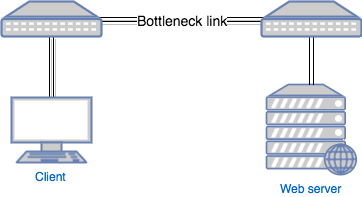
\includegraphics[width=0.7\textwidth]{../master-thesis/figures/testbench.pdf}}

    \end{overprint}

\end{frame}

% ------------------------------------

\begin{frame}
    \frametitle{My testbench}
    %\framesubtitle{}

    \begin{overprint}

        \uncover<+->{\center\includegraphics[width=1.1\textwidth]{../master-thesis/figures/testbed-workflow.pdf}}

    \end{overprint}

\end{frame}

% ------------------------------------

\begin{frame}
    \frametitle{My testbench}
    \framesubtitle{The content loaded over the network}

    \begin{overprint}
        \uncover<+->{}

        \uncover<+->{Loads pre-downloaded content from 42 of Alexas top 100 webpages over a virtualized bottleneck link.}
        ~\\
        ~\\
        \uncover<+->{Measures network load times and how much data the browser managed to fetch.}
        ~\\
        ~\\
        \uncover<+->{Uses 16 different scenarios, each tested with both a persistent connection as well as a new connection for each page load.} \note{Scenario here means different properties of the bottleneck link.}

    \end{overprint}

\end{frame}

% ------------------------------------

\begin{frame}
    \frametitle{My testbench}
    \framesubtitle{Scenario categories}

    \begin{overprint}
        \uncover<+->{}
        \begin{itemize}
                \uncover<+->{
                \item Baseline}
                \uncover<+->{
                \item Bandwidth limited}
                \uncover<+->{
                \item Latency added}
                \uncover<+->{
                \item Loss added}
        \end{itemize}
    \end{overprint}

\end{frame}
